%% AASTeX v7+ calls the following external packages:
%% times, hyperref, ifthen, hyphens, longtable, xcolor, 
%% bookmarks, array, rotating, ulem, and lineno 
\documentclass[twocolumn]{aastex701}

\usepackage{booktabs}
\usepackage[table]{xcolor}
\usepackage{colortbl}
\usepackage{natbib}
\usepackage{float}

\begin{document}

\title{LLM Influence on Physics and Astrophysics Writing: Vocabulary Shifts in arXiv Abstracts}

\author[orcid=0000-0003-4105-3443]{Elisha Modelevsky}
\affiliation{Racah Institute of Physics, Hebrew University of Jerusalem}
\email[show]{elisha.modelevsky@mail.huji.ac.il}  

%% Mark off the abstract in the ``abstract'' environment. 
\begin{abstract}

Large language models (LLMs) have been rapidly adopted across scientific workflows, and their influence on scientific work has been observed in many studies.
We quantify changes in vocabulary usage in arXiv abstracts by analyzing astrophysics subcategories (astro-ph.CO/EP/GA/HE/IM/SR) alongside other physics areas (cond-mat, hep, nucl) and computer science (cs).
Using the arXiv API, we collect up to 250 abstracts per month per category from January 2019 through June 2025, and measure frequencies for a curated list of terms that are commonly associated with LLM-generated text, along with some comparison terms.
We calculate the post-ChatGPT factor increase relative to a pre-ChatGPT baseline (threshold December 2022) for each category, and assess significance with z-tests.
We find statistically significant increases in LLM-favored vocabulary across all domains after the introduction of ChatGPT, with the greatest change in computer science.
Physics categories exhibit more modest increases, without major differences between them, except for a lower baseline in High Energy and Nuclear Physics.
Differences among astrophysics subfields are even less significant.


\end{abstract}

% \keywords{\uat{Galaxies}{573}}
%% You can use the \uat command to link your UAT concepts back its source.
% \keywords{\uat{Galaxies}{573} --- \uat{Cosmology}{343} --- \uat{High Energy astrophysics}{739} --- \uat{Interstellar medium}{847} --- \uat{Stellar astronomy}{1583} --- \uat{Solar physics}{1476}}

\section{Introduction} 

ChatGPT was introduced on 30 November 2022 by OpenAI as a revolutionary large language model (LLM), capable of understanding and generating human-like text \citep{Roumeliotis2023}.
Since its release, many other LLMs with similar capabilities have emerged, and these models are now widely used for various tasks, including writing and coding \citep{Minaee2024}.
The influence of LLMs on science is an ongoing discussion -- while they can be very useful and efficient for many stages in the scientific process, some researchers express concerns about the potential for misuse and the impact on scientific integrity \citep{Zhang2025}.

Another aspect of science where the footprint of LLMs is very apparent is scientific writing.
Previous studies have demonstrated linguistic shifts in scientific language;
notably, some studies have found a significant increase in the use of certain words and phrases since the introduction of ChatGPT \citep{Kobak2025,Bao2025,Juzek2024}.
An interesting phenomenon highlighted by \citet{Lin2025} is the ``equalization'' of scientific language across countries of origin, characterized by a reduction in linguistic differences between native and non-native English-speaking authors.

Prior studies have investigated linguistic shifts in general scientific writing and in select disciplines \citep{Xu2024,Kobak2025,Bao2025}, but to our knowledge, a systematic analysis focusing specifically on astrophysics has not yet been conducted.
This work aims to fill this gap by examining the change in vocubalary in astrophysics abstracts since the introduction of ChatGPT, and comparing it to other branches of physics.
We also investigate whether different subfields within astrophysics have been affected differently.


\section{Methods}

To gather the data, we use the arXiv API to collect abstracts from papers in each of the astrophysics subcategories (astro-ph.CO/EP/GA/HE/IM/SR) and several other physics categories (cond-mat, hep, nucl) as well as Computer Science (cs).
Due to API limitations, we collect a maximum of 250 abstracts per month from each category, spanning from January 2019 to June 2025.

In each abstract, we count the occurrences of each word in a predefined list of words (see Table~\ref{tab:factor_increase} for the word list).
The words in this list are those that have been commonly cited as overused by LLMs \citep{Bao2025,Kobak2025}, as well as some words that are not expected to be overused.
The usage statistics are aggregated by yearly quarters and arXiv category.
Figure~\ref{fig:word_usage_trends_example} shows an example of the usage trends of several words in the astro-ph category.

To determine the factor increase in word usage, we calculate the ratio of the frequency of each word in abstracts after the introduction of ChatGPT to its frequency before.
We then perform a z-test to assess the statistical significance of the change in frequency for each word.


\section{Results}

Table~\ref{tab:factor_increase} shows statistically significant factor increases in word usage after the introduction of ChatGPT, broken down by arXiv category.
Similarly to previous findings \citep{Juzek2024,Bao2025,Kobak2025}, words such as ``delve'', ``leverage'', ``intricate'', ``valuable'' and ``pivotal'' have seen a significant increase in usage across all categories.
However, some words that were reported as overused, such as ``foster'', ``boast'', ``remarkable'', ``thereby'' and ``innovative'' have seen a significant increase in only some of the categories.
In particular, all of these words' usage has increased significantly in the Computer Science category, but not in all of the physics categories.

Regarding the different astrophysics subcategories, no particular trend was observed to distinguish between them.

We identify words that are strong suspects of being overused due to LLMs by looking for words that have seen a significant increase in usage of at least 50\% in at least 3 of the major categories (astro-ph, cond-mat, hep, nucl, cs).
These words appear in Table~\ref{tab:factor_increase} in boldface.
To quantify the overall influence of LLMs on scientific writing in each category, we define an \emph{``LLM influence score''} as number of appearances of these strong suspect words per abstract.

Figures~\ref{fig:category_comparison} and \ref{fig:astro_subcat_comparison} show the LLM influence score over time in different arXiv categories and astro-ph subcategories, respectively.
While there is no clear difference between the astrophysics subcategories, it seems that LLM-favored words were always more prevalent in astro-ph.IM (Instrumentation and Methods for Astrophysics) and in astro-ph.EP (Earth and Planetary Astrophysics).

The category comparison in Figure~\ref{fig:category_comparison} reveals that the Computer Science category has been the most affected by LLMs, with a significant increase in the LLM influence score after the introduction of ChatGPT.
That remains true even after subtracting the baseline of LLM-favored words usage, which was higher in Computer Science abstracts than in physics even before the introduction of ChatGPT.

Table~\ref{tab:expected_words_per_abstract_before_after} shows the expected number of LLM-favored words per abstract in each category, before and after the introduction of ChatGPT.
Besides the clear strong influence on Computer Science, it can be seen that the in the changes in physics categories are more modest, and are similar to one another.
Interestingly, High Energy Physics (hep) and Nuclear Physics (nucl) have had a lower baseline (LLM-favored word usage prior to ChatGPT) than Condensed Matter Physics (cond-mat) and Astrophysics (astro-ph).


\begin{figure}[h]
\centering
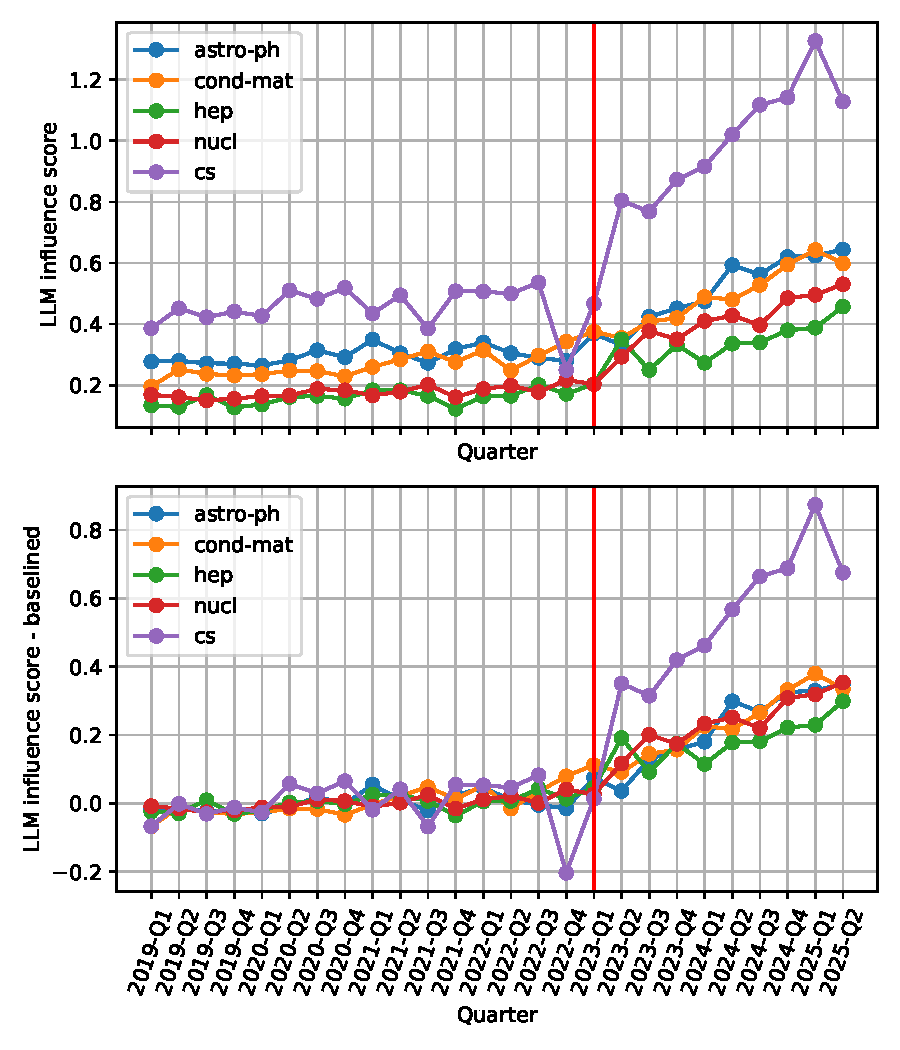
\includegraphics[width=\columnwidth]{scripts/figs/major_cats_score_vs_time.pdf}
\caption{
LLM influence score over time in different arXiv categories.
The bottom panel shows the baselined score (the score minus the average score before ChatGPT).
The red vertical line indicates the introduction of ChatGPT (2022-Q4).
}
\label{fig:category_comparison}
\end{figure}

\begin{figure}[h]
\centering
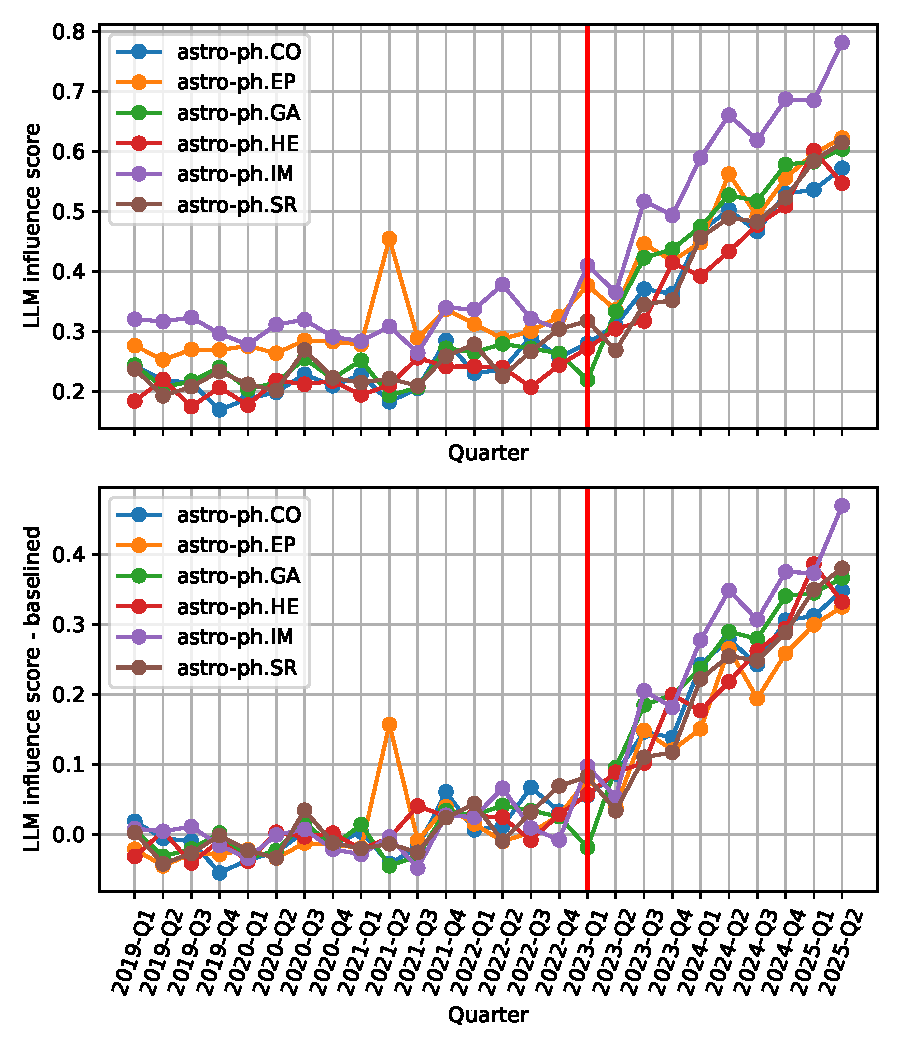
\includegraphics[width=\columnwidth]{scripts/figs/astro_subcats_score_vs_time.pdf}
\caption{
LLM influence score over time in different astro-ph subcategories.
The bottom panel shows the baselined score (the score minus the average score before ChatGPT).
The red vertical line indicates the introduction of ChatGPT (2022-Q4).
}
\label{fig:astro_subcat_comparison}
\end{figure}

\begin{table}
\centering
\begin{tabular}{lccc}
\toprule
Category & Before & After & Difference \\
\midrule
astro-ph & 0.294 & 0.509 & 0.215 \\
cond-mat & 0.267 & 0.490 & 0.223 \\
hep & 0.160 & 0.346 & 0.186 \\
nucl & 0.177 & 0.398 & 0.221 \\
cs & 0.462 & 1.053 & 0.591 \\
\bottomrule
\end{tabular}
\caption{Expected number of LLM-favored words per abstract in each category, before and after the introduction of ChatGPT.}
\label{tab:expected_words_per_abstract_before_after}
\end{table}


\section{Summary \& Discussion}

We analyzed vocabulary shifts in arXiv abstracts (from January 2019 to June 2025) across astrophysics subcategories, other physics (cond-mat, hep, nucl), and computer science.
In this study, we investigated the impact of large language models (LLMs) on the vocabulary used in arXiv abstracts across astrophysics subcategories, several physics categories, and computer science.
Our analysis revealed a significant increase in the usage of LLM-favored words in all categories following the introduction of ChatGPT.
Computer science is the most strongly affected, whereas the physics categories show more modest increases that are similar to one another -- though High Energy Physics and Nuclear Physics have a lower baseline than Astrophysics and Condensed Matter Physics.
No significant differences were observed between the astrophysics subcategories.

Future investigations could expand the vocabulary list to include more words and phrases associated with LLM-generated text, and could also analyze the full text of papers rather than just abstracts.
In particular, a known effect of LLMs is the increased usage of em-dashes, which was not included in this study after it was found that abstracts rarely include em-dashes.
A more thorough analysis should be able to estimate more confidently the percentage of papers that were written with the help of LLMs, and how that percentage varies across disciplines -- potentially revealing more pronounced effects than what we have been able to observe.


\section*{Acknowledgments}
The author thanks his colleague Nadav Shoval for helpful discussions and comments.

\bibliography{references}{}
\bibliographystyle{aasjournalv7}

\appendix 
\renewcommand{\thesection}{\Alph{section}}
\renewcommand{\thefigure}{\Alph{section}\arabic{figure}}
\renewcommand{\thetable}{\Alph{section}\arabic{table}}

\section{Example word usage trends}
\setcounter{figure}{0}
\setcounter{table}{0}

\begin{figure*}[ht]
\centering
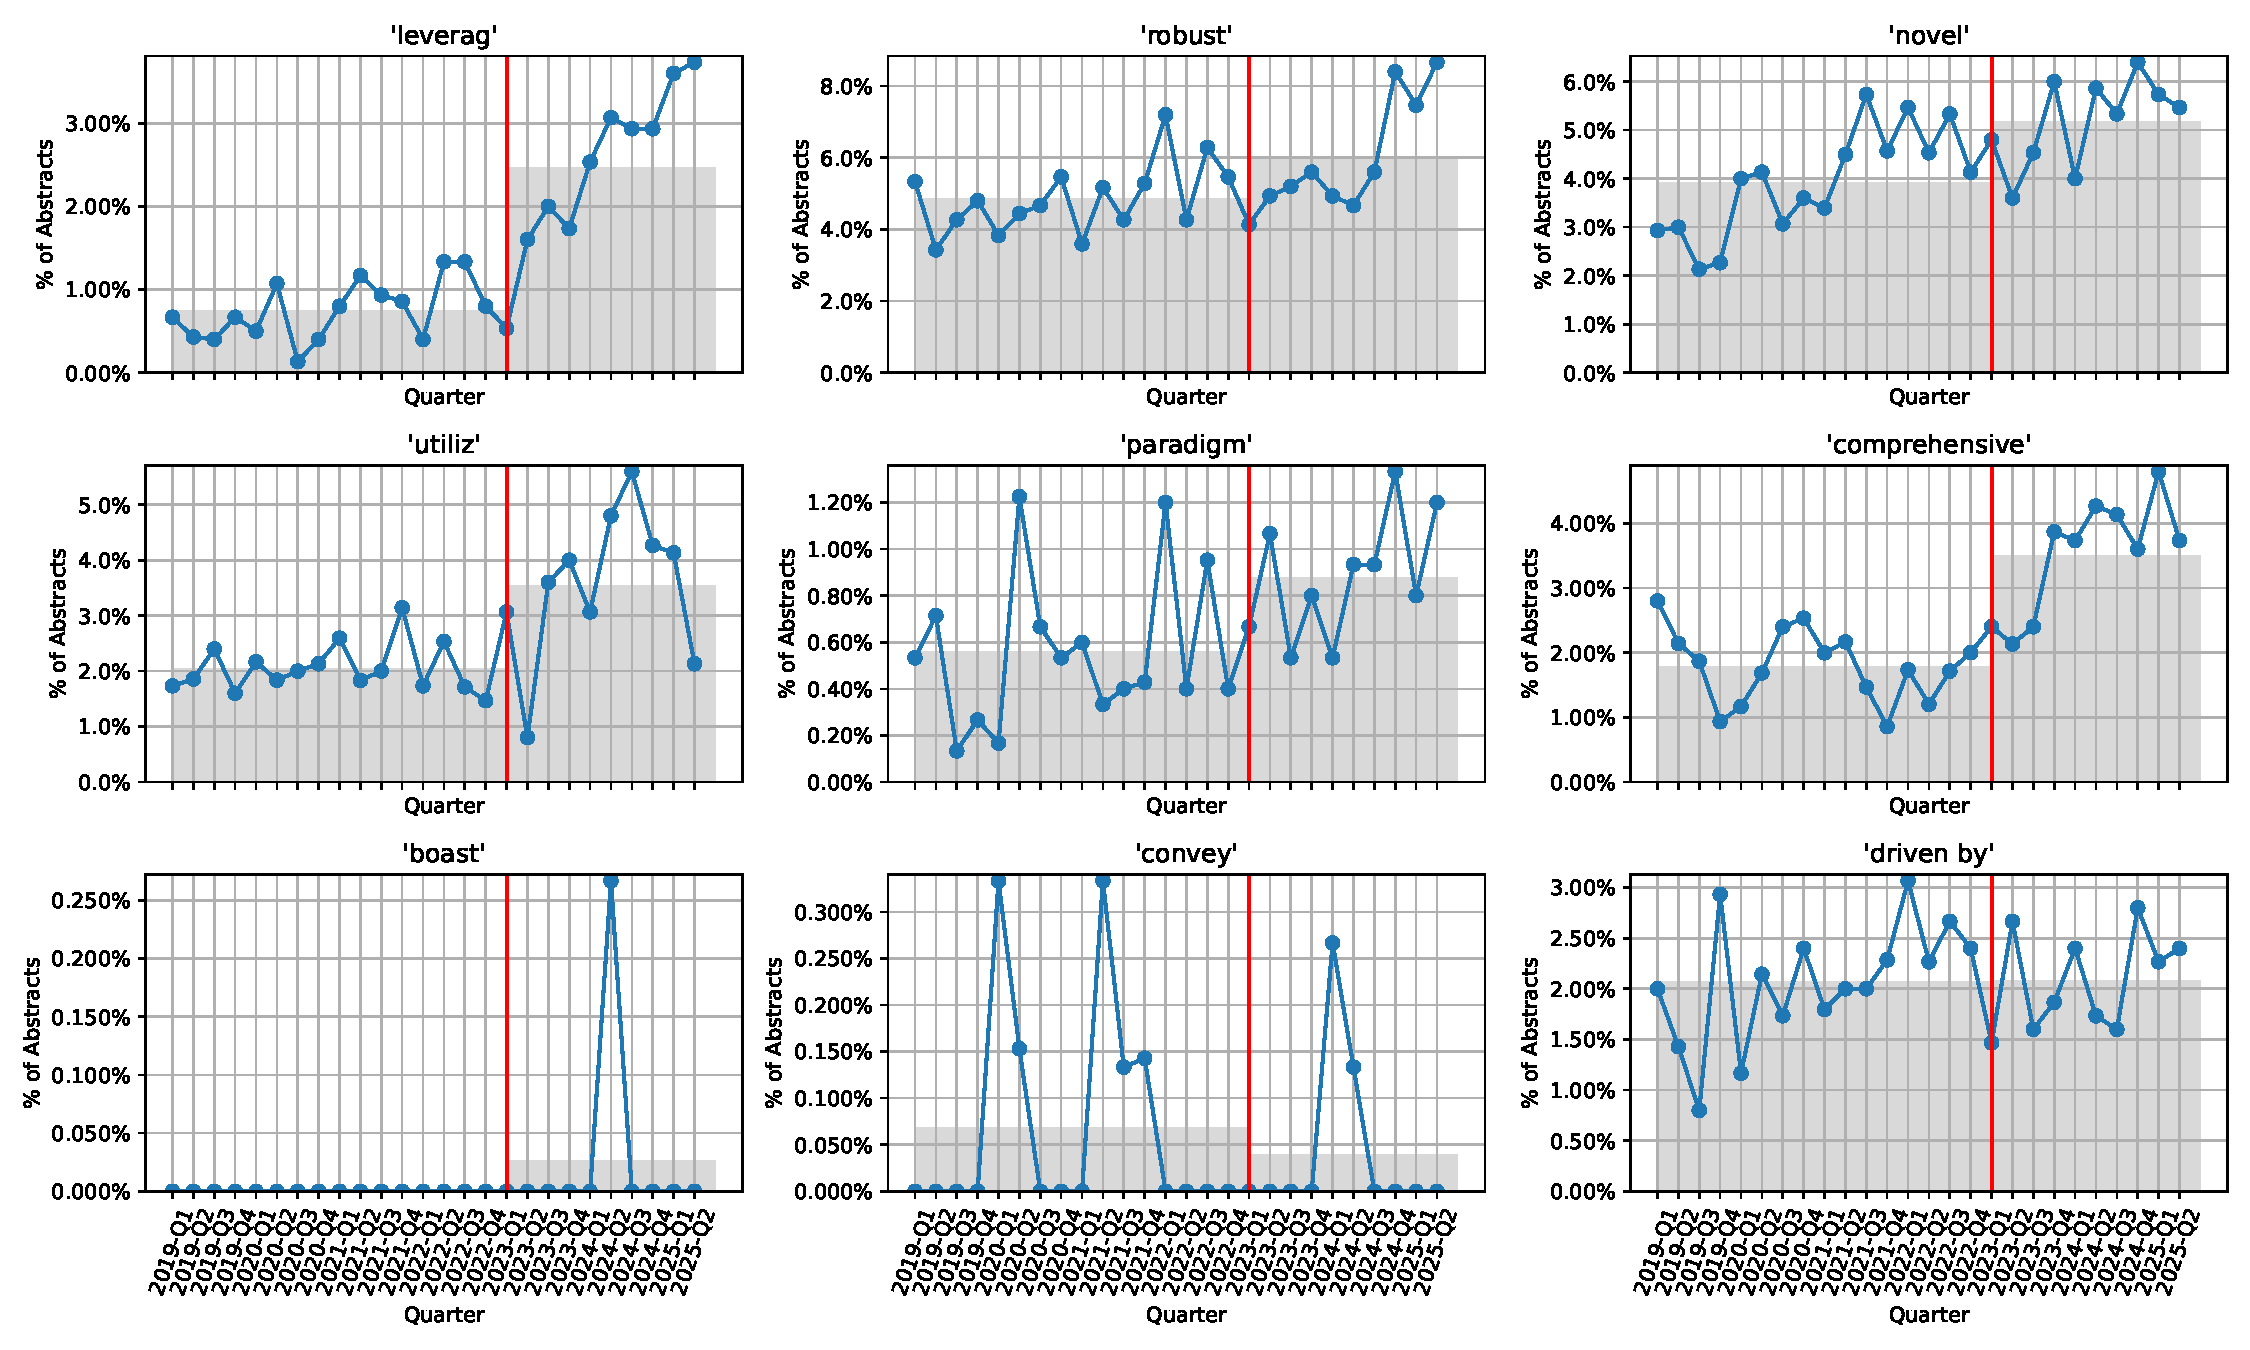
\includegraphics[width=\textwidth]{scripts/figs/example_usage_vs_time_astro-ph.pdf}
\caption{
Example of word usage trends over time in the astro-ph category -- the fraction of abstracts containing each word is plotted over time (in quarters).
The red vertical line indicates the introduction of ChatGPT (2022-Q4).
The gray shaded area reprensents the mean fraction before and after the introduction of ChatGPT.
}
\label{fig:word_usage_trends_example}
\end{figure*}

\section{Factor increase table for all words and categories}
\setcounter{figure}{0}
\setcounter{table}{0}

\begin{table*}[ht]
\centering
\scriptsize
\setlength{\tabcolsep}{3pt}
\begin{tabular}{|l|c|c|c|c|c|c|c|c|c|c|c|}
\toprule
 & astro-ph.CO & astro-ph.EP & astro-ph.GA & astro-ph.HE & astro-ph.IM & astro-ph.SR & astro-ph & cond-mat & hep & nucl & cs \\
Word &  &  &  &  &  &  &  &  &  &  &  \\
\midrule
additionally & \cellcolor{yellow!53} 2.68 & \cellcolor{yellow!38} 1.90 & \cellcolor{yellow!46} 2.31 & \cellcolor{yellow!46} 2.30 & \cellcolor{yellow!38} 1.90 & \cellcolor{yellow!44} 2.20 & \cellcolor{yellow!37} 1.87 & \cellcolor{yellow!46} 2.31 & \cellcolor{yellow!72} 3.63 & \cellcolor{yellow!65} 3.27 & \cellcolor{yellow!47} 2.38 \\
albeit &  &  &  &  &  &  &  & \cellcolor{yellow!35} 1.77 & \cellcolor{yellow!38} 1.91 &  &  \\
boast &  &  &  &  &  &  &  &  &  &  & \cellcolor{yellow!100} 7.00 \\
capabilities &  &  & \cellcolor{yellow!28} 1.44 &  & \cellcolor{yellow!27} 1.36 & \cellcolor{yellow!28} 1.42 & \cellcolor{yellow!25} 1.27 &  &  &  & \cellcolor{yellow!52} 2.64 \\
change &  & \cellcolor{yellow!17} 0.89 &  &  &  &  & \cellcolor{yellow!17} 0.89 &  &  & \cellcolor{yellow!23} 1.15 &  \\
comprehensive & \cellcolor{yellow!39} 1.97 & \cellcolor{yellow!36} 1.81 & \cellcolor{yellow!38} 1.90 & \cellcolor{yellow!41} 2.07 & \cellcolor{yellow!46} 2.30 & \cellcolor{yellow!32} 1.63 & \cellcolor{yellow!39} 1.95 & \cellcolor{yellow!40} 2.00 & \cellcolor{yellow!42} 2.14 & \cellcolor{yellow!41} 2.07 & \cellcolor{yellow!57} 2.90 \\
critical & \cellcolor{yellow!24} 1.23 & \cellcolor{yellow!23} 1.15 & \cellcolor{yellow!25} 1.26 & \cellcolor{yellow!24} 1.20 & \cellcolor{yellow!23} 1.17 & \cellcolor{yellow!23} 1.17 &  &  & \cellcolor{yellow!24} 1.22 &  & \cellcolor{yellow!36} 1.83 \\
crucial & \cellcolor{yellow!34} 1.70 & \cellcolor{yellow!32} 1.64 & \cellcolor{yellow!38} 1.91 & \cellcolor{yellow!33} 1.68 & \cellcolor{yellow!36} 1.83 & \cellcolor{yellow!34} 1.70 & \cellcolor{yellow!34} 1.74 & \cellcolor{yellow!27} 1.35 & \cellcolor{yellow!31} 1.55 & \cellcolor{yellow!40} 2.01 & \cellcolor{yellow!48} 2.43 \\
delv & \cellcolor{yellow!100} 5.67 & \cellcolor{yellow!100} 7.50 & \cellcolor{yellow!80} 4.00 & \cellcolor{yellow!100} 8.00 & \cellcolor{yellow!100} 5.80 & \cellcolor{yellow!100} 9.00 & \cellcolor{yellow!80} 4.00 & \cellcolor{yellow!100} 28.00 & \cellcolor{yellow!100} 6.33 &  & \cellcolor{yellow!100} 6.90 \\
discover &  & \cellcolor{yellow!17} 0.87 & \cellcolor{yellow!23} 1.19 & \cellcolor{yellow!22} 1.10 &  &  &  & \cellcolor{yellow!24} 1.24 &  &  & \cellcolor{yellow!24} 1.21 \\
driven by & \cellcolor{yellow!25} 1.25 & \cellcolor{yellow!25} 1.26 &  & \cellcolor{yellow!25} 1.29 &  &  &  & \cellcolor{yellow!25} 1.28 &  &  & \cellcolor{yellow!53} 2.69 \\
effectively & \cellcolor{yellow!31} 1.55 &  & \cellcolor{yellow!41} 2.07 & \cellcolor{yellow!30} 1.54 & \cellcolor{yellow!36} 1.83 & \cellcolor{yellow!30} 1.52 & \cellcolor{yellow!31} 1.57 & \cellcolor{yellow!27} 1.38 & \cellcolor{yellow!43} 2.16 & \cellcolor{yellow!35} 1.78 & \cellcolor{yellow!41} 2.09 \\
endeavor &  &  &  &  &  &  &  &  &  & \cellcolor{yellow!68} 3.40 &  \\
enhance & \cellcolor{yellow!28} 1.41 & \cellcolor{yellow!24} 1.20 &  &  & \cellcolor{yellow!41} 2.07 &  & \cellcolor{yellow!29} 1.48 & \cellcolor{yellow!22} 1.14 & \cellcolor{yellow!25} 1.29 & \cellcolor{yellow!27} 1.40 & \cellcolor{yellow!78} 3.93 \\
exceptional & \cellcolor{yellow!33} 1.67 &  & \cellcolor{yellow!31} 1.59 & \cellcolor{yellow!31} 1.56 & \cellcolor{yellow!40} 2.02 & \cellcolor{yellow!29} 1.48 & \cellcolor{yellow!30} 1.54 & \cellcolor{yellow!26} 1.32 &  & \cellcolor{yellow!57} 2.88 & \cellcolor{yellow!57} 2.86 \\
find & \cellcolor{yellow!21} 1.08 & \cellcolor{yellow!21} 1.07 & \cellcolor{yellow!21} 1.06 & \cellcolor{yellow!21} 1.07 & \cellcolor{yellow!22} 1.11 & \cellcolor{yellow!21} 1.08 & \cellcolor{yellow!21} 1.05 & \cellcolor{yellow!23} 1.16 &  & \cellcolor{yellow!23} 1.17 & \cellcolor{yellow!24} 1.21 \\
foster &  &  &  &  &  &  &  &  & \cellcolor{yellow!100} 7.67 & \cellcolor{yellow!66} 3.33 & \cellcolor{yellow!75} 3.75 \\
framework & \cellcolor{yellow!29} 1.47 & \cellcolor{yellow!26} 1.33 & \cellcolor{yellow!27} 1.35 & \cellcolor{yellow!27} 1.35 & \cellcolor{yellow!33} 1.69 & \cellcolor{yellow!26} 1.30 & \cellcolor{yellow!29} 1.49 & \cellcolor{yellow!29} 1.48 & \cellcolor{yellow!26} 1.30 & \cellcolor{yellow!25} 1.29 & \cellcolor{yellow!30} 1.54 \\
groundbreaking &  &  &  &  &  &  & \cellcolor{yellow!60} 3.00 & \cellcolor{yellow!100} 6.50 &  &  & \cellcolor{yellow!100} 5.17 \\
help &  & \cellcolor{yellow!24} 1.20 &  &  &  &  &  &  &  &  & \cellcolor{yellow!17} 0.86 \\
in-depth &  &  &  &  &  & \cellcolor{yellow!35} 1.75 &  & \cellcolor{yellow!44} 2.21 & \cellcolor{yellow!60} 3.00 &  &  \\
innovative &  & \cellcolor{yellow!45} 2.26 &  &  & \cellcolor{yellow!26} 1.33 &  &  & \cellcolor{yellow!80} 4.00 &  & \cellcolor{yellow!38} 1.92 & \cellcolor{yellow!87} 4.37 \\
insight & \cellcolor{yellow!50} 2.53 & \cellcolor{yellow!36} 1.84 & \cellcolor{yellow!46} 2.30 & \cellcolor{yellow!47} 2.35 & \cellcolor{yellow!35} 1.77 & \cellcolor{yellow!50} 2.53 & \cellcolor{yellow!38} 1.92 & \cellcolor{yellow!39} 1.98 & \cellcolor{yellow!46} 2.30 & \cellcolor{yellow!37} 1.89 & \cellcolor{yellow!45} 2.29 \\
intricate & \cellcolor{yellow!77} 3.86 & \cellcolor{yellow!63} 3.17 & \cellcolor{yellow!100} 8.17 & \cellcolor{yellow!100} 9.60 & \cellcolor{yellow!100} 13.33 & \cellcolor{yellow!61} 3.07 & \cellcolor{yellow!100} 5.71 & \cellcolor{yellow!49} 2.49 & \cellcolor{yellow!78} 3.90 & \cellcolor{yellow!100} 9.80 & \cellcolor{yellow!100} 6.28 \\
leverag & \cellcolor{yellow!89} 4.47 & \cellcolor{yellow!60} 3.03 & \cellcolor{yellow!91} 4.58 & \cellcolor{yellow!100} 5.21 & \cellcolor{yellow!73} 3.66 & \cellcolor{yellow!85} 4.26 & \cellcolor{yellow!67} 3.38 & \cellcolor{yellow!70} 3.50 & \cellcolor{yellow!90} 4.52 & \cellcolor{yellow!100} 5.67 & \cellcolor{yellow!53} 2.67 \\
look &  &  &  &  &  & \cellcolor{yellow!26} 1.30 &  &  &  &  &  \\
make &  &  &  & \cellcolor{yellow!15} 0.77 &  &  &  & \cellcolor{yellow!16} 0.80 &  & \cellcolor{yellow!16} 0.84 & \cellcolor{yellow!16} 0.83 \\
need &  &  &  &  &  &  & \cellcolor{yellow!22} 1.11 &  &  &  & \cellcolor{yellow!23} 1.17 \\
notabl & \cellcolor{yellow!52} 2.60 & \cellcolor{yellow!40} 2.01 & \cellcolor{yellow!57} 2.89 & \cellcolor{yellow!56} 2.82 & \cellcolor{yellow!49} 2.49 & \cellcolor{yellow!43} 2.18 & \cellcolor{yellow!39} 1.99 & \cellcolor{yellow!58} 2.92 & \cellcolor{yellow!47} 2.38 & \cellcolor{yellow!92} 4.63 & \cellcolor{yellow!54} 2.70 \\
novel & \cellcolor{yellow!26} 1.34 & \cellcolor{yellow!27} 1.39 & \cellcolor{yellow!31} 1.55 & \cellcolor{yellow!30} 1.50 & \cellcolor{yellow!27} 1.39 & \cellcolor{yellow!29} 1.48 & \cellcolor{yellow!26} 1.33 &  & \cellcolor{yellow!24} 1.22 & \cellcolor{yellow!28} 1.41 & \cellcolor{yellow!27} 1.38 \\
paradigm & \cellcolor{yellow!26} 1.30 & \cellcolor{yellow!32} 1.64 &  &  &  &  & \cellcolor{yellow!32} 1.60 &  &  & \cellcolor{yellow!32} 1.64 & \cellcolor{yellow!30} 1.53 \\
paramount &  &  & \cellcolor{yellow!53} 2.67 &  &  &  &  & \cellcolor{yellow!55} 2.75 &  &  & \cellcolor{yellow!34} 1.73 \\
particularly & \cellcolor{yellow!33} 1.69 & \cellcolor{yellow!30} 1.53 & \cellcolor{yellow!34} 1.73 & \cellcolor{yellow!34} 1.72 & \cellcolor{yellow!32} 1.65 & \cellcolor{yellow!27} 1.40 & \cellcolor{yellow!31} 1.55 & \cellcolor{yellow!32} 1.63 & \cellcolor{yellow!28} 1.45 & \cellcolor{yellow!36} 1.84 & \cellcolor{yellow!50} 2.51 \\
pivotal & \cellcolor{yellow!61} 3.08 & \cellcolor{yellow!100} 5.22 & \cellcolor{yellow!75} 3.77 & \cellcolor{yellow!40} 2.00 & \cellcolor{yellow!94} 4.73 & \cellcolor{yellow!50} 2.50 & \cellcolor{yellow!67} 3.36 & \cellcolor{yellow!64} 3.22 & \cellcolor{yellow!74} 3.73 & \cellcolor{yellow!78} 3.93 & \cellcolor{yellow!100} 6.35 \\
primarily & \cellcolor{yellow!27} 1.35 & \cellcolor{yellow!30} 1.50 & \cellcolor{yellow!33} 1.67 & \cellcolor{yellow!31} 1.59 &  & \cellcolor{yellow!31} 1.57 & \cellcolor{yellow!27} 1.37 & \cellcolor{yellow!45} 2.27 & \cellcolor{yellow!39} 1.98 & \cellcolor{yellow!46} 2.33 & \cellcolor{yellow!51} 2.57 \\
promising & \cellcolor{yellow!27} 1.38 & \cellcolor{yellow!26} 1.34 &  &  & \cellcolor{yellow!23} 1.18 &  & \cellcolor{yellow!27} 1.39 & \cellcolor{yellow!27} 1.35 & \cellcolor{yellow!25} 1.27 & \cellcolor{yellow!30} 1.54 & \cellcolor{yellow!35} 1.79 \\
remarkable & \cellcolor{yellow!29} 1.49 &  & \cellcolor{yellow!29} 1.48 &  &  &  &  &  &  &  & \cellcolor{yellow!57} 2.88 \\
rigorous & \cellcolor{yellow!29} 1.48 &  &  &  &  &  &  &  & \cellcolor{yellow!29} 1.47 &  &  \\
robust & \cellcolor{yellow!27} 1.38 & \cellcolor{yellow!24} 1.20 & \cellcolor{yellow!27} 1.36 & \cellcolor{yellow!25} 1.29 & \cellcolor{yellow!29} 1.46 & \cellcolor{yellow!23} 1.19 & \cellcolor{yellow!24} 1.22 & \cellcolor{yellow!26} 1.30 & \cellcolor{yellow!28} 1.41 & \cellcolor{yellow!33} 1.68 & \cellcolor{yellow!37} 1.86 \\
scalable & \cellcolor{yellow!44} 2.22 &  &  &  & \cellcolor{yellow!36} 1.83 &  & \cellcolor{yellow!47} 2.39 & \cellcolor{yellow!40} 2.03 & \cellcolor{yellow!84} 4.20 &  & \cellcolor{yellow!26} 1.30 \\
show & \cellcolor{yellow!18} 0.94 &  &  & \cellcolor{yellow!19} 0.95 &  &  & \cellcolor{yellow!18} 0.94 & \cellcolor{yellow!18} 0.93 & \cellcolor{yellow!18} 0.91 &  & \cellcolor{yellow!17} 0.85 \\
significant & \cellcolor{yellow!24} 1.21 & \cellcolor{yellow!24} 1.22 & \cellcolor{yellow!24} 1.21 & \cellcolor{yellow!24} 1.23 & \cellcolor{yellow!27} 1.38 & \cellcolor{yellow!23} 1.15 & \cellcolor{yellow!24} 1.22 & \cellcolor{yellow!32} 1.61 & \cellcolor{yellow!28} 1.43 & \cellcolor{yellow!27} 1.36 & \cellcolor{yellow!37} 1.86 \\
small &  & \cellcolor{yellow!18} 0.93 & \cellcolor{yellow!18} 0.91 & \cellcolor{yellow!17} 0.87 & \cellcolor{yellow!17} 0.89 &  & \cellcolor{yellow!17} 0.85 & \cellcolor{yellow!17} 0.87 &  &  &  \\
state-of-the-art &  & \cellcolor{yellow!27} 1.36 &  &  & \cellcolor{yellow!24} 1.23 & \cellcolor{yellow!27} 1.39 &  &  & \cellcolor{yellow!27} 1.38 & \cellcolor{yellow!24} 1.23 & \cellcolor{yellow!25} 1.25 \\
subsequently & \cellcolor{yellow!32} 1.62 &  &  &  & \cellcolor{yellow!32} 1.60 & \cellcolor{yellow!28} 1.45 & \cellcolor{yellow!28} 1.42 &  &  &  & \cellcolor{yellow!37} 1.87 \\
systematic & \cellcolor{yellow!23} 1.15 &  &  &  &  &  & \cellcolor{yellow!23} 1.16 & \cellcolor{yellow!25} 1.26 & \cellcolor{yellow!23} 1.19 & \cellcolor{yellow!24} 1.20 & \cellcolor{yellow!31} 1.55 \\
thereby &  &  & \cellcolor{yellow!37} 1.87 &  & \cellcolor{yellow!32} 1.60 &  &  & \cellcolor{yellow!30} 1.53 & \cellcolor{yellow!31} 1.57 & \cellcolor{yellow!33} 1.67 & \cellcolor{yellow!40} 2.04 \\
thoroughly &  &  &  &  & \cellcolor{yellow!44} 2.21 &  &  &  &  &  &  \\
uncover & \cellcolor{yellow!54} 2.74 & \cellcolor{yellow!30} 1.53 & \cellcolor{yellow!48} 2.41 & \cellcolor{yellow!42} 2.10 &  & \cellcolor{yellow!32} 1.63 &  & \cellcolor{yellow!31} 1.56 & \cellcolor{yellow!35} 1.79 &  & \cellcolor{yellow!37} 1.88 \\
unveil & \cellcolor{yellow!45} 2.28 & \cellcolor{yellow!37} 1.88 & \cellcolor{yellow!34} 1.71 &  &  &  & \cellcolor{yellow!35} 1.76 & \cellcolor{yellow!32} 1.63 &  &  &  \\
utiliz & \cellcolor{yellow!49} 2.45 & \cellcolor{yellow!32} 1.61 & \cellcolor{yellow!54} 2.72 & \cellcolor{yellow!48} 2.44 & \cellcolor{yellow!35} 1.79 & \cellcolor{yellow!49} 2.47 & \cellcolor{yellow!34} 1.74 & \cellcolor{yellow!36} 1.81 & \cellcolor{yellow!49} 2.49 & \cellcolor{yellow!49} 2.46 & \cellcolor{yellow!37} 1.85 \\
valuable & \cellcolor{yellow!43} 2.17 & \cellcolor{yellow!35} 1.75 & \cellcolor{yellow!44} 2.23 & \cellcolor{yellow!43} 2.17 & \cellcolor{yellow!43} 2.16 & \cellcolor{yellow!43} 2.19 & \cellcolor{yellow!35} 1.79 & \cellcolor{yellow!65} 3.28 & \cellcolor{yellow!50} 2.52 & \cellcolor{yellow!38} 1.94 & \cellcolor{yellow!47} 2.39 \\
vital &  & \cellcolor{yellow!32} 1.65 & \cellcolor{yellow!35} 1.76 & \cellcolor{yellow!32} 1.63 & \cellcolor{yellow!33} 1.68 & \cellcolor{yellow!31} 1.57 &  & \cellcolor{yellow!36} 1.84 & \cellcolor{yellow!53} 2.69 & \cellcolor{yellow!46} 2.32 & \cellcolor{yellow!32} 1.61 \\
\bottomrule
\end{tabular}

\caption{
Factor increase in word usage since the introduction of ChatGPT (threshold December 2022), by arXiv category.
Blank cells indicate non-significant changes ($p \geq 0.05$).
The color scale indicates the magnitude of the factor increase, with darker green representing larger increases, and darker red representing larger decreases.
The words in boldface are those that have seen a significant increase of at least 50\% in at least 3 of the 5 major categories.
Note that the words ``delv'', ``leverag'', and ``utiliz'' are stemmed to include all their morphological variants (e.g., ``delve'' and ``delving'').
}
\label{tab:factor_increase}
\end{table*}

\end{document}
